\documentclass[11pt]{article}
\usepackage[margin=1in]{geometry}
\usepackage{graphicx}
\usepackage{microtype}
\usepackage{verbatim}
\usepackage{amsmath}
\usepackage{nicefrac}
\usepackage[colorlinks=false, hidelinks]{hyperref}
\usepackage{caption}
\usepackage{subcaption}
\usepackage{listings}
\usepackage{harmony}
\usepackage{wasysym}

\begin{document}

\title{The Last Music Trainer\\Embedded System Design, Lab 4}
\date{October 8, 2015}
\author{Ben Lorenzetti}
\maketitle

\tableofcontents

\clearpage

\section{Objectives and Problem Descriptions}
\subsection{Beginner Music Trainer}
\label{problem-specs}

The objective of this lab is to develop microcontroller-based, beginner music trainer 
with the following features:
\begin{enumerate}

\item Be capable of playing simple songs using PBasic's 
\mbox{\texttt{FREQOUT Pin, Duraction, Freq1 \{, Freq2\}}} command.
This including the ability to
\begin{enumerate}
\item[a.] play any piano tone in the $4^{\textrm{th}}$--$7^{\textrm{th}}$ octave
\{C, C\#, D, D\#, E, F, F\#, G, G\#, A, A\#, B\};

\item[b.] change the base tempo's whole note duration;

\item[c.] play each note for \{1, $\nicefrac{1}{2}$, $\nicefrac{1}{4}$, $\nicefrac{1}{8}$,
$\nicefrac{1}{16}$, $\nicefrac{1}{32}$\} of the base tempo;

\item[d.] play each note for $1\frac{1}{2}*\{1$, $\nicefrac{1}{2}$, $\nicefrac{1}{4}$, $\nicefrac{1}{8}$, 
$\nicefrac{1}{16}$, $\nicefrac{1}{32}$\} (dotten notes) of the base tempo; and
\end{enumerate}

\item allow user to select from a menu of 5 Ring Tone Text Transfer Language
(RTTTL) songs,
using a pushbutton switch--each push causes an advance to the next song.

\item allow user to increase the base tempo by a factor of 1--4 using a potentiometer rotary knob.

\item display the current note being played on a 7-segment display,
using the decimal point to indicate sharp notes.
Furthermore, display the note's octave with individual LEDs.

\item play each song in an infinite loop if user does not advance to the next song.
\end{enumerate}

\section{Procedure}
\subsection{Circuit Design}

\begin{figure}[h!]
\centering
	\begin{subfigure}[b]{.2\textwidth}
		\centering
		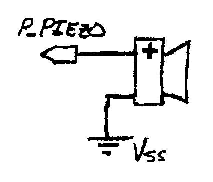
\includegraphics[width=\textwidth]{piezo-circuit.pdf}
		\caption[]%
		{{\small Piezo Circuit}}
	\end{subfigure}
	\quad
	\begin{subfigure}[b]{0.45\textwidth}
		\centering
		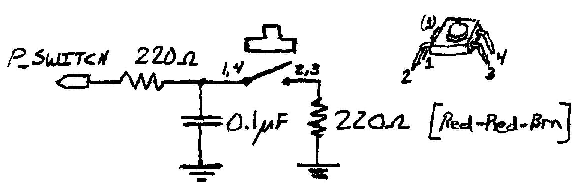
\includegraphics[width=\textwidth]{pushbutton-circuit.pdf}
		\caption[]%
		{{Pushbutton Switch Circuit}}
	\end{subfigure}
	\vskip\baselineskip
	\begin{subfigure}[b]{0.45\textwidth}
		\centering
		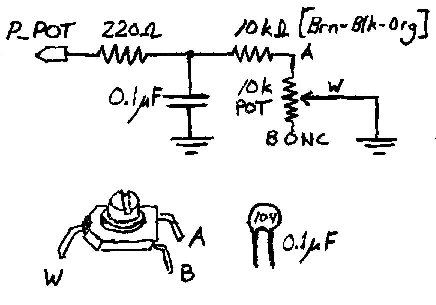
\includegraphics[width=\textwidth]{potentiometer-circuit.pdf}
		\caption[]%
		{{Potentiometer RC Circiut}}
	\end{subfigure}
	\quad
	\begin{subfigure}[b]{0.45\textwidth}
		\centering
		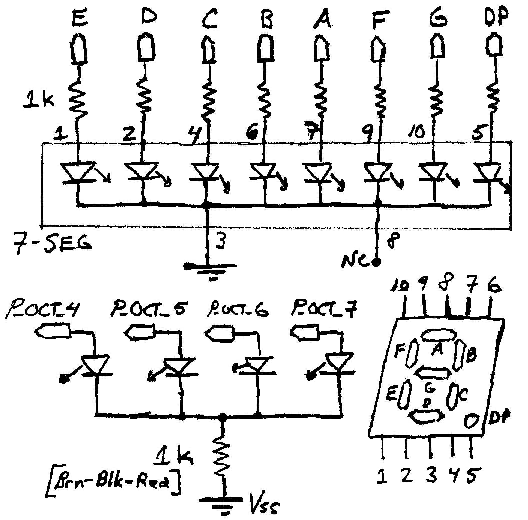
\includegraphics[width=\textwidth]{LED-display-circuit.pdf}
		\caption[]%
		{{LED Display Circuit}}
	\end{subfigure}	
	\caption{Hardware for The Last Music Trainer}
	\label{circuit-diagrams}
\end{figure}

\subsection{Data Design}

\begin{center}
\includegraphics[width=.4\textwidth]{one-byte-data-analysis.pdf}
\label{one-byte-data-breakdown}
\end{center}

\begin{table}
\centering
\caption{10-Bit Note Encoding Truth Table}
\resizebox{\textwidth}{!}{
\begin{tabular}{c | c c | c | c | c | c c | c | c}
\hline
Length				&$*$	&Bit Code	&Dec.	&Whole Note Divisor	&Letter		&\#	&Bit Code	&Dec.	&$7^{\textrm{th}}$ Octave Freq	\\
\hline\hline
{\Huge \fullnote \par}		&0	&000		&0	&$(1<<0)$		&A$\natural$	&0	&000		&0	&3520.0	\\
\hline
{\Huge \fullnote \Pu \par}	&1	&000		&8	&			&A$\sharp$	&1	&000		&8	&3729.3	\\
\hline
{\Huge \halfnote \par}		&0	&001		&1	&$(1<<1)$		&B$\natural$	&0	&001		&1	&3951.1	\\
\hline
{\Huge \halfnote \Pu \par}	&1	&001		&9	&			&C$\natural$	&0	&010		&2	&2093.0	\\
\hline
{\Huge \quarternote \par}	&0	&010		&2	&$(1<<2)$		&C$\sharp$	&1	&010		&10	&2217.5	\\
\hline
{\Huge \quarternote \Pu \par}	&1	&010		&10	&			&D$\natural$	&0	&011		&3	&2349.3	\\
\hline
{\Huge \Acht \par}		&0	&011		&3	&$(1<<3)$		&D$\sharp$	&1	&011		&11	&2489.0	\\
\hline
{\Huge \Acht \Pu \par}		&1	&011		&11	&			&E$\natural$	&0	&100		&4	&2637.0	\\
\hline
{\Huge \Sech \par}		&0	&100		&4	&$(1<<4)$		&F$\natural$	&0	&101		&5	&2793.8	\\
\hline
{\Huge \Sech \Pu \par}		&1	&100		&12	&			&F$\sharp$	&1	&101		&13	&2960.0	\\
\hline
{\Huge \Zwdr \par}		&0	&101		&5	&$(1<<5)$		&G$\natural$	&0	&110		&6	&3136.0	\\
\hline
{\Huge \Zwdr \Pu \par}		&1	&101		&13	&			&G$\sharp$	&1	&110		&14	&3322.4	\\
\hline
				&	&		&	&			&P	&x	&111		&7,15	&-\\
\hline\hline
&&&&&	Octave				&	&Bit Code	&Dec.	&$7^{\textrm{th}}$ Freq. Divisor	\\
\hline\hline
&&&&&	$4^{\textrm{th}}$		&	&00		&0	&$1<<(3-0)$	\\
&&&&&	$5^{\textrm{th}}$		&	&01		&1	&$1<<(3-1)$	\\
&&&&&	$6^{\textrm{th}}$		&	&10		&2	&$1<<(3-2)$	\\
&&&&&	$7^{\textrm{th}}$		&	&11		&3	&$1<<(3-3)$	\\
\hline
\end{tabular}}
\label{data-lookup-table}
\end{table}

\subsection{Data Generation from RTTTL Files}

\subsection{Implementation Flowchart}

\begin{figure}[h!]
\centering
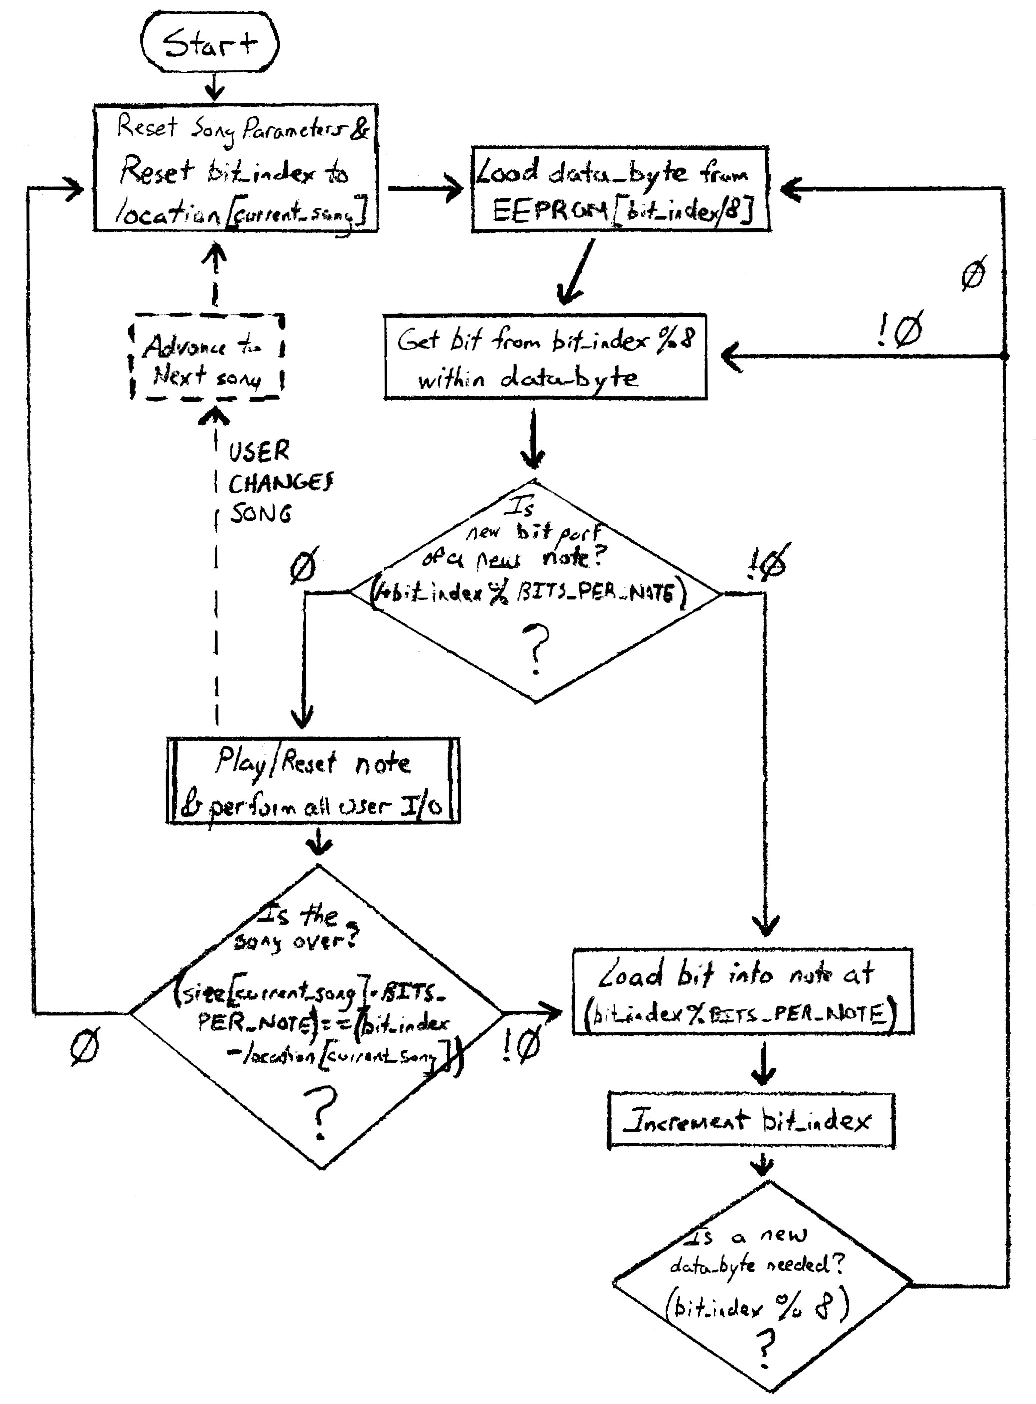
\includegraphics[width=0.8\textwidth]{music-trainer-flowchart.pdf}
\caption{Music Trainer Implementation Flowchart}
\label{music-trainer-flowchart}
\end{figure}

\section{Expected Results}

\subsection{Why is this a section?}
I expected my microcontroller and circuit to behave as described in
\hyperref[problem-specs]{section \ref{problem-specs}}.
Not going to waste paper by copying the specifications here...

\section{Experiment and Design Revisions}

\section{Observations}

\begin{figure}[h!]
\centering
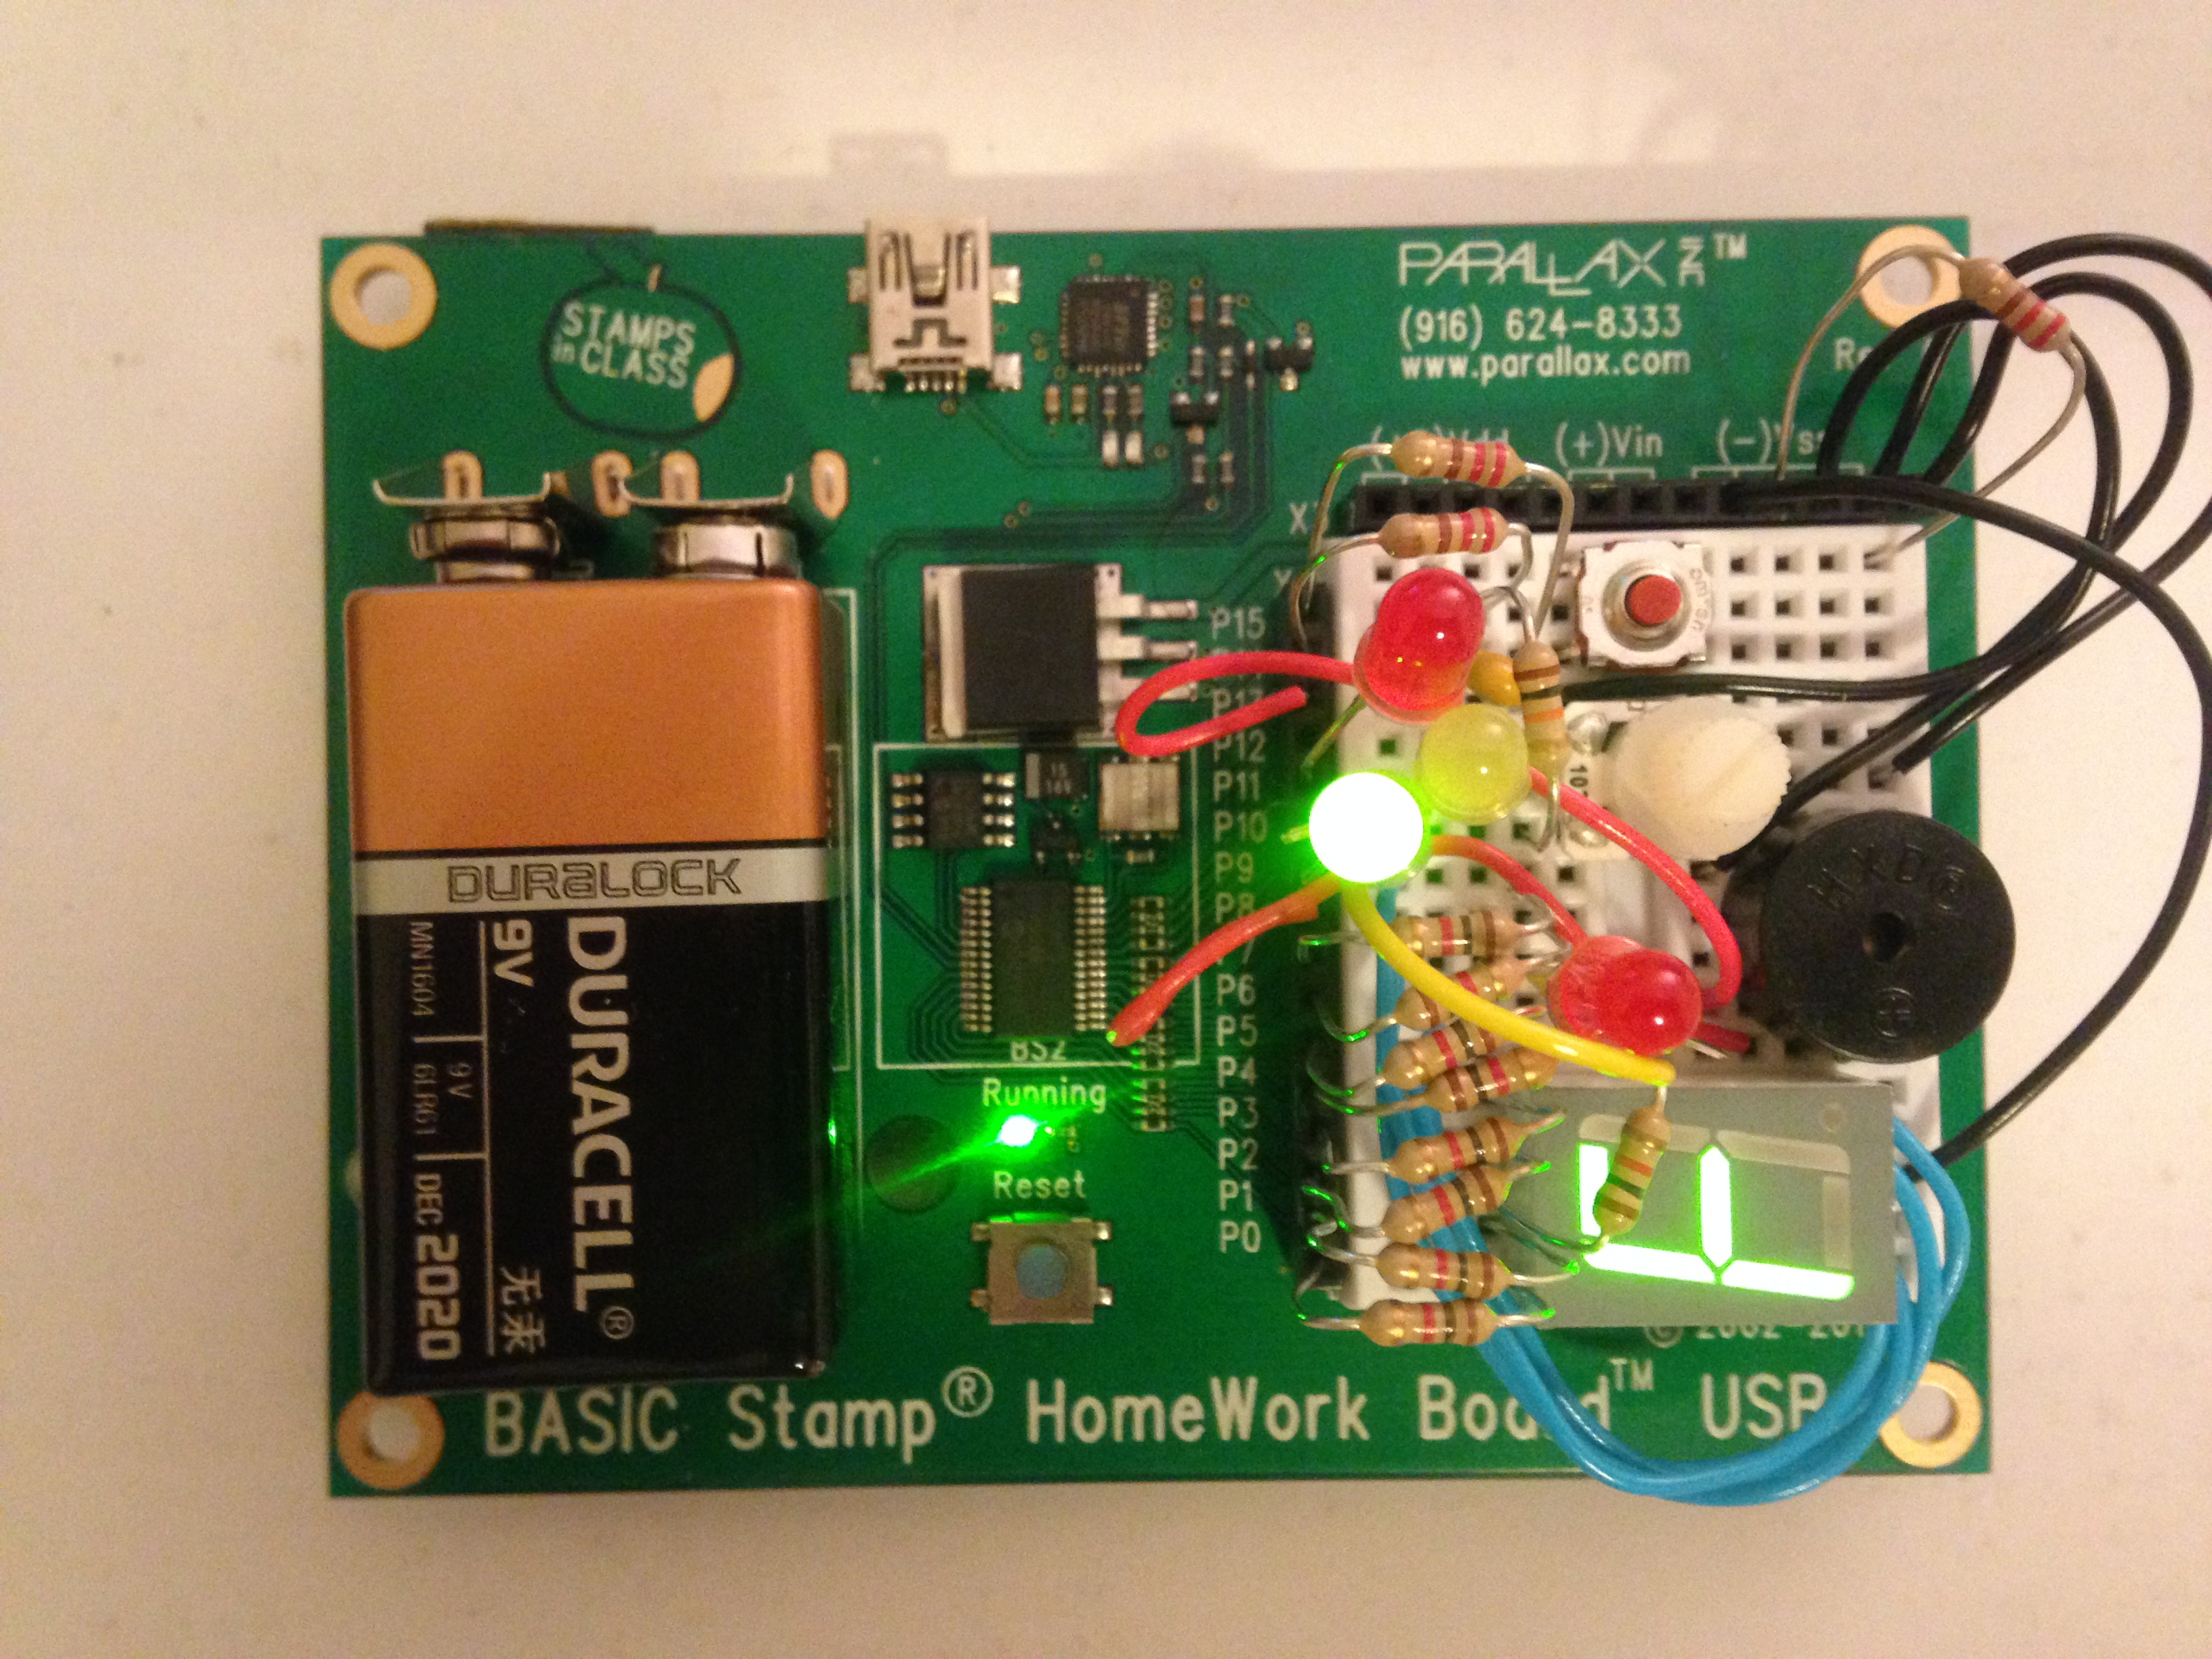
\includegraphics[width=0.6\textwidth]{the-music-trainer.jpg}
\caption{My Music Trainer Playing The Final Countdown}
\label{the-music-trainer}
\end{figure}

\begin{figure}[h!]
\centering
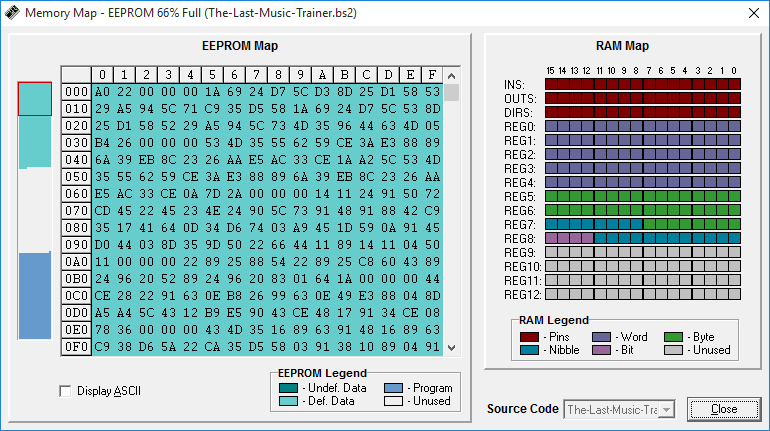
\includegraphics[width=\textwidth]{memory-map.png}
\caption{EEPROM Memory Mapping with Six Songs}
\label{memory-map}
\end{figure}

\section{Discussion}

\section{Exercises}

\clearpage

\section{Implementation Code}

\subsection{The-Last-Music-Trainer.bs2}

\begingroup
\fontsize{10pt}{12pt}
\verbatiminput{The-Last-Music-Trainer.bs2}
\endgroup

\clearpage
\subsection{generate-rtttl-song-data.c}

\lstinputlisting[breaklines]{generate-rtttl-song-data.c}



\end{document}
